\documentclass{article}
\usepackage{tikz}
\usetikzlibrary{arrows.meta}

\begin{document}

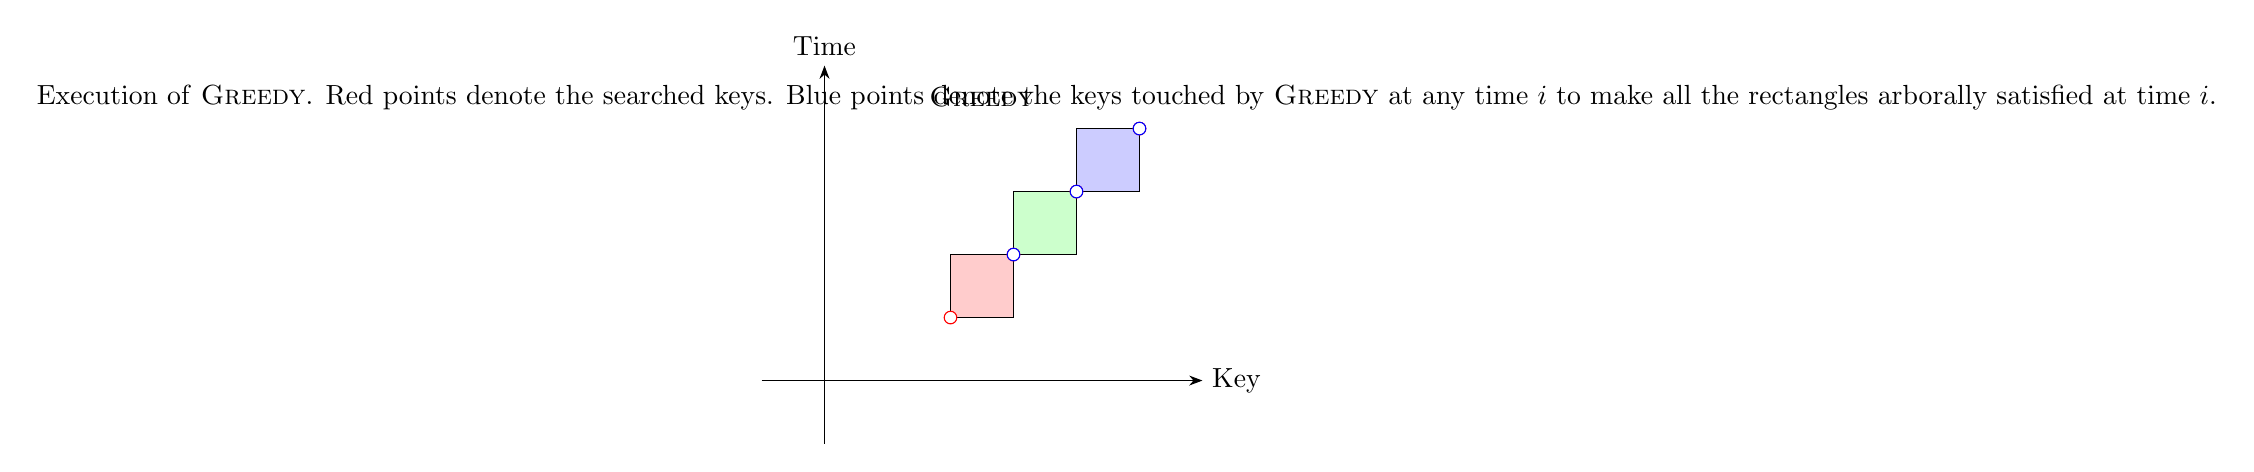
\begin{tikzpicture}[scale=0.8, >=Stealth]
    % Draw axes
    \draw[->] (-1,0) -- (6,0) node[right] {Key};
    \draw[->] (0,-1) -- (0,5) node[above] {Time};

    % Draw rectangles with red points and blue points
    \filldraw[draw=black, fill=red!20] (2,1) rectangle (3,2);
    \filldraw[draw=black, fill=green!20] (3,2) rectangle (4,3);
    \filldraw[draw=black, fill=blue!20] (4,3) rectangle (5,4);

    \filldraw[draw=red, fill=white] (2,1) circle (0.1); % Red point
    \filldraw[draw=red, fill=white] (3,2) circle (0.1); % Red point
    \filldraw[draw=red, fill=white] (4,3) circle (0.1); % Red point
    \filldraw[draw=red, fill=white] (5,4) circle (0.1); % Red point

    \filldraw[draw=blue, fill=white] (3,2) circle (0.1); % Blue point
    \filldraw[draw=blue, fill=white] (4,3) circle (0.1); % Blue point
    \filldraw[draw=blue, fill=white] (5,4) circle (0.1); % Blue point

    % Draw text annotations
    \node at (2.5, 4.5) {\textsc{Greedy}};
    \node at (4.8, 4.5) {Execution of \textsc{Greedy}. Red points denote the searched keys. Blue points denote the keys touched by \textsc{Greedy} at any time $i$ to make all the rectangles arborally satisfied at time $i$.};
\end{tikzpicture}

\end{document}